

\tikzset{every picture/.style={line width=0.75pt}} %set default line width to 0.75pt        

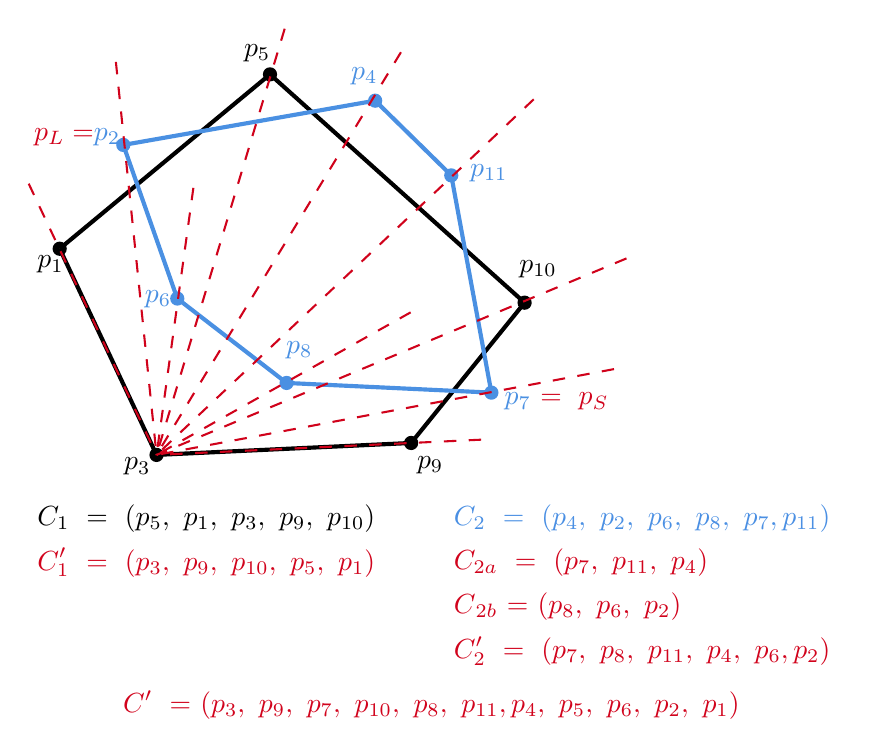
\begin{tikzpicture}[x=0.5pt,y=0.5pt,yscale=-1,xscale=1]
%uncomment if require: \path (0,506); %set diagram left start at 0, and has height of 506

%Flowchart: Connector [id:dp3760201615823463] 
\draw  [fill={rgb, 255:red, 0; green, 0; blue, 0 }  ,fill opacity=1 ] (57,162) .. controls (57,159.58) and (58.96,157.62) .. (61.38,157.62) .. controls (63.79,157.62) and (65.75,159.58) .. (65.75,162) .. controls (65.75,164.42) and (63.79,166.38) .. (61.38,166.38) .. controls (58.96,166.38) and (57,164.42) .. (57,162) -- cycle ;
%Flowchart: Connector [id:dp5854006172506206] 
\draw  [fill={rgb, 255:red, 0; green, 0; blue, 0 }  ,fill opacity=1 ] (209,36) .. controls (209,33.58) and (210.96,31.62) .. (213.38,31.62) .. controls (215.79,31.62) and (217.75,33.58) .. (217.75,36) .. controls (217.75,38.42) and (215.79,40.38) .. (213.38,40.38) .. controls (210.96,40.38) and (209,38.42) .. (209,36) -- cycle ;
%Flowchart: Connector [id:dp03971004338552875] 
\draw  [fill={rgb, 255:red, 0; green, 0; blue, 0 }  ,fill opacity=1 ] (311,302.38) .. controls (311,299.96) and (312.96,298) .. (315.38,298) .. controls (317.79,298) and (319.75,299.96) .. (319.75,302.38) .. controls (319.75,304.79) and (317.79,306.75) .. (315.38,306.75) .. controls (312.96,306.75) and (311,304.79) .. (311,302.38) -- cycle ;
%Flowchart: Connector [id:dp4369716280602779] 
\draw  [fill={rgb, 255:red, 0; green, 0; blue, 0 }  ,fill opacity=1 ] (127,311) .. controls (127,308.58) and (128.96,306.62) .. (131.38,306.62) .. controls (133.79,306.62) and (135.75,308.58) .. (135.75,311) .. controls (135.75,313.42) and (133.79,315.38) .. (131.38,315.38) .. controls (128.96,315.38) and (127,313.42) .. (127,311) -- cycle ;
%Flowchart: Connector [id:dp03888777155399348] 
\draw  [color={rgb, 255:red, 74; green, 144; blue, 226 }  ,draw opacity=1 ][fill={rgb, 255:red, 74; green, 144; blue, 226 }  ,fill opacity=1 ] (103,87) .. controls (103,84.58) and (104.96,82.62) .. (107.38,82.62) .. controls (109.79,82.62) and (111.75,84.58) .. (111.75,87) .. controls (111.75,89.42) and (109.79,91.38) .. (107.38,91.38) .. controls (104.96,91.38) and (103,89.42) .. (103,87) -- cycle ;
%Flowchart: Connector [id:dp6352844555884073] 
\draw  [fill={rgb, 255:red, 0; green, 0; blue, 0 }  ,fill opacity=1 ] (393,201) .. controls (393,198.58) and (394.96,196.62) .. (397.38,196.62) .. controls (399.79,196.62) and (401.75,198.58) .. (401.75,201) .. controls (401.75,203.42) and (399.79,205.38) .. (397.38,205.38) .. controls (394.96,205.38) and (393,203.42) .. (393,201) -- cycle ;
%Flowchart: Connector [id:dp23645115309917453] 
\draw  [color={rgb, 255:red, 74; green, 144; blue, 226 }  ,draw opacity=1 ][fill={rgb, 255:red, 74; green, 144; blue, 226 }  ,fill opacity=1 ] (285,55) .. controls (285,52.58) and (286.96,50.62) .. (289.38,50.62) .. controls (291.79,50.62) and (293.75,52.58) .. (293.75,55) .. controls (293.75,57.42) and (291.79,59.38) .. (289.38,59.38) .. controls (286.96,59.38) and (285,57.42) .. (285,55) -- cycle ;
%Straight Lines [id:da9582823916987413] 
\draw [color={rgb, 255:red, 0; green, 0; blue, 0 }  ,draw opacity=1 ][line width=1.5]    (131.38,311) -- (315.38,302.38) ;
%Straight Lines [id:da7170032735395258] 
\draw [color={rgb, 255:red, 0; green, 0; blue, 0 }  ,draw opacity=1 ][line width=1.5]    (61.38,162) -- (213.38,36) ;
%Straight Lines [id:da7153530187498507] 
\draw [color={rgb, 255:red, 0; green, 0; blue, 0 }  ,draw opacity=1 ][fill={rgb, 255:red, 245; green, 166; blue, 35 }  ,fill opacity=1 ][line width=1.5]    (61.38,162) -- (92.84,228.96) -- (131.38,311) ;
%Straight Lines [id:da6087381521295036] 
\draw [color={rgb, 255:red, 0; green, 0; blue, 0 }  ,draw opacity=1 ][line width=1.5]    (213.38,36) -- (397.38,201) ;
%Straight Lines [id:da7334727922272425] 
\draw [color={rgb, 255:red, 0; green, 0; blue, 0 }  ,draw opacity=1 ][line width=1.5]    (315.38,302.38) -- (397.38,201) ;
%Flowchart: Connector [id:dp3946295929267337] 
\draw  [color={rgb, 255:red, 74; green, 144; blue, 226 }  ,draw opacity=1 ][fill={rgb, 255:red, 74; green, 144; blue, 226 }  ,fill opacity=1 ] (142,198) .. controls (142,195.58) and (143.96,193.62) .. (146.38,193.62) .. controls (148.79,193.62) and (150.75,195.58) .. (150.75,198) .. controls (150.75,200.42) and (148.79,202.38) .. (146.38,202.38) .. controls (143.96,202.38) and (142,200.42) .. (142,198) -- cycle ;
%Flowchart: Connector [id:dp5536782520392832] 
\draw  [color={rgb, 255:red, 74; green, 144; blue, 226 }  ,draw opacity=1 ][fill={rgb, 255:red, 74; green, 144; blue, 226 }  ,fill opacity=1 ] (221,259) .. controls (221,256.58) and (222.96,254.62) .. (225.38,254.62) .. controls (227.79,254.62) and (229.75,256.58) .. (229.75,259) .. controls (229.75,261.42) and (227.79,263.38) .. (225.38,263.38) .. controls (222.96,263.38) and (221,261.42) .. (221,259) -- cycle ;
%Flowchart: Connector [id:dp5354107395187737] 
\draw  [color={rgb, 255:red, 74; green, 144; blue, 226 }  ,draw opacity=1 ][fill={rgb, 255:red, 74; green, 144; blue, 226 }  ,fill opacity=1 ] (369,266) .. controls (369,263.58) and (370.96,261.62) .. (373.38,261.62) .. controls (375.79,261.62) and (377.75,263.58) .. (377.75,266) .. controls (377.75,268.42) and (375.79,270.38) .. (373.38,270.38) .. controls (370.96,270.38) and (369,268.42) .. (369,266) -- cycle ;
%Flowchart: Connector [id:dp21529891001736134] 
\draw  [color={rgb, 255:red, 74; green, 144; blue, 226 }  ,draw opacity=1 ][fill={rgb, 255:red, 74; green, 144; blue, 226 }  ,fill opacity=1 ] (340,109) .. controls (340,106.58) and (341.96,104.62) .. (344.38,104.62) .. controls (346.79,104.62) and (348.75,106.58) .. (348.75,109) .. controls (348.75,111.42) and (346.79,113.38) .. (344.38,113.38) .. controls (341.96,113.38) and (340,111.42) .. (340,109) -- cycle ;
%Straight Lines [id:da13610377148087538] 
\draw [color={rgb, 255:red, 74; green, 144; blue, 226 }  ,draw opacity=1 ][line width=1.5]    (146.38,198) -- (107.38,87) ;
%Straight Lines [id:da17098738082940423] 
\draw [color={rgb, 255:red, 74; green, 144; blue, 226 }  ,draw opacity=1 ][line width=1.5]    (373.38,266) -- (225.38,259) ;
%Straight Lines [id:da39885017452703897] 
\draw [color={rgb, 255:red, 74; green, 144; blue, 226 }  ,draw opacity=1 ][line width=1.5]    (373.38,266) -- (344.38,109) ;
%Straight Lines [id:da49076142701312997] 
\draw [color={rgb, 255:red, 74; green, 144; blue, 226 }  ,draw opacity=1 ][line width=1.5]    (344.38,109) -- (289.38,55) ;
%Straight Lines [id:da7133961892030377] 
\draw [color={rgb, 255:red, 74; green, 144; blue, 226 }  ,draw opacity=1 ][line width=1.5]    (225.38,259) -- (146.38,198) ;
%Straight Lines [id:da6192417354090246] 
\draw [color={rgb, 255:red, 74; green, 144; blue, 226 }  ,draw opacity=1 ][line width=1.5]    (289.38,55) -- (107.38,87) ;
%Straight Lines [id:da3354599107667824] 
\draw [color={rgb, 255:red, 208; green, 2; blue, 27 }  ,draw opacity=1 ][line width=0.75]  [dash pattern={on 4.5pt off 4.5pt}]  (462,249) -- (131.38,311) ;
%Straight Lines [id:da37383354135177016] 
\draw [color={rgb, 255:red, 208; green, 2; blue, 27 }  ,draw opacity=1 ][line width=0.75]  [dash pattern={on 4.5pt off 4.5pt}]  (315,208) -- (131.38,311) ;
%Straight Lines [id:da663432735093426] 
\draw [color={rgb, 255:red, 208; green, 2; blue, 27 }  ,draw opacity=1 ][line width=0.75]  [dash pattern={on 4.5pt off 4.5pt}]  (404,54) -- (131.38,311) ;
%Straight Lines [id:da4154054026142908] 
\draw [color={rgb, 255:red, 208; green, 2; blue, 27 }  ,draw opacity=1 ][line width=0.75]  [dash pattern={on 4.5pt off 4.5pt}]  (308,20) -- (131.38,311) ;
%Straight Lines [id:da9171997534785323] 
\draw [color={rgb, 255:red, 208; green, 2; blue, 27 }  ,draw opacity=1 ][line width=0.75]  [dash pattern={on 4.5pt off 4.5pt}]  (102,27) -- (131.38,311) ;
%Straight Lines [id:da9698007508961525] 
\draw [color={rgb, 255:red, 208; green, 2; blue, 27 }  ,draw opacity=1 ][line width=0.75]  [dash pattern={on 4.5pt off 4.5pt}]  (224,3) -- (131.38,311) ;
%Straight Lines [id:da3710951051522332] 
\draw [color={rgb, 255:red, 208; green, 2; blue, 27 }  ,draw opacity=1 ][line width=0.75]  [dash pattern={on 4.5pt off 4.5pt}]  (158,118) -- (131.38,311) ;
%Straight Lines [id:da8247371840671284] 
\draw [color={rgb, 255:red, 208; green, 2; blue, 27 }  ,draw opacity=1 ][line width=0.75]  [dash pattern={on 4.5pt off 4.5pt}]  (471,169) -- (131.38,311) ;
%Straight Lines [id:da3258545016218505] 
\draw [color={rgb, 255:red, 208; green, 2; blue, 27 }  ,draw opacity=1 ][line width=0.75]  [dash pattern={on 4.5pt off 4.5pt}]  (366,300) -- (131.38,311) ;
%Straight Lines [id:da24778748747353996] 
\draw [color={rgb, 255:red, 208; green, 2; blue, 27 }  ,draw opacity=1 ][line width=0.75]  [dash pattern={on 4.5pt off 4.5pt}]  (39,115) -- (131.38,311) ;

% Text Node
\draw (43,345) node [anchor=north west][inner sep=0.75pt]   [align=left] {$\displaystyle C_{1} \ =\ ( p_{5} ,\ p_{1} ,\ p_{3} ,\ p_{9} ,\ p_{10}) \ $};
% Text Node
\draw (43,165) node [anchor=north west][inner sep=0.75pt]   [align=left] {$\displaystyle p_{1}$};
% Text Node
\draw (40.75,73) node [anchor=north west][inner sep=0.75pt]  [color={rgb, 255:red, 74; green, 144; blue, 226 }  ,opacity=1 ] [align=left] {$\displaystyle \textcolor[rgb]{0.82,0.01,0.11}{p_{L} =} p_{2}$};
% Text Node
\draw (269.75,29) node [anchor=north west][inner sep=0.75pt]  [color={rgb, 255:red, 74; green, 144; blue, 226 }  ,opacity=1 ] [align=left] {$\displaystyle p_{4}$};
% Text Node
\draw (120.75,190) node [anchor=north west][inner sep=0.75pt]  [color={rgb, 255:red, 74; green, 144; blue, 226 }  ,opacity=1 ] [align=left] {$\displaystyle p_{6}$};
% Text Node
\draw (380.75,264) node [anchor=north west][inner sep=0.75pt]  [color={rgb, 255:red, 74; green, 144; blue, 226 }  ,opacity=1 ] [align=left] {$\displaystyle p_{7} \ \textcolor[rgb]{0.82,0.01,0.11}{=\ p_{S}}$};
% Text Node
\draw (105.75,311) node [anchor=north west][inner sep=0.75pt]   [align=left] {$\displaystyle p_{3}$};
% Text Node
\draw (317.38,309.75) node [anchor=north west][inner sep=0.75pt]   [align=left] {$\displaystyle p_{9}$};
% Text Node
\draw (391.38,168.38) node [anchor=north west][inner sep=0.75pt]   [align=left] {$\displaystyle p_{10}$};
% Text Node
\draw (192.38,12.38) node [anchor=north west][inner sep=0.75pt]   [align=left] {$\displaystyle p_{5}$};
% Text Node
\draw (222.75,227) node [anchor=north west][inner sep=0.75pt]  [color={rgb, 255:red, 74; green, 144; blue, 226 }  ,opacity=1 ] [align=left] {$\displaystyle p_{8}$};
% Text Node
\draw (355.75,99) node [anchor=north west][inner sep=0.75pt]  [color={rgb, 255:red, 74; green, 144; blue, 226 }  ,opacity=1 ] [align=left] {$\displaystyle p_{11}$};
% Text Node
\draw (344,345) node [anchor=north west][inner sep=0.75pt]   [align=left] {$\displaystyle \textcolor[rgb]{0.29,0.56,0.89}{C_{2} \ =\ ( p_{4} ,\ p_{2} ,\ p_{6} ,\ p_{8} ,\ p_{7} ,p_{11}) \ }$};
% Text Node
\draw (344,376.67) node [anchor=north west][inner sep=0.75pt]   [align=left] {$\displaystyle \textcolor[rgb]{0.82,0.01,0.11}{C_{2a} \ =\ ( p_{7} ,\ p_{11} ,\ p_{4}) \ }$};
% Text Node
\draw (344,408.34) node [anchor=north west][inner sep=0.75pt]   [align=left] {$\displaystyle \textcolor[rgb]{0.82,0.01,0.11}{C}\textcolor[rgb]{0.82,0.01,0.11}{_{2b}}\textcolor[rgb]{0.82,0.01,0.11}{\ =\ }\textcolor[rgb]{0.82,0.01,0.11}{(}\textcolor[rgb]{0.82,0.01,0.11}{p}\textcolor[rgb]{0.82,0.01,0.11}{_{8}}\textcolor[rgb]{0.82,0.01,0.11}{,\ p}\textcolor[rgb]{0.82,0.01,0.11}{_{6}}\textcolor[rgb]{0.82,0.01,0.11}{,\ p}\textcolor[rgb]{0.82,0.01,0.11}{_{2}}\textcolor[rgb]{0.82,0.01,0.11}{)}\textcolor[rgb]{0.82,0.01,0.11}{\ }$};
% Text Node
\draw (344,440) node [anchor=north west][inner sep=0.75pt]   [align=left] {$\displaystyle \textcolor[rgb]{0.82,0.01,0.11}{C'_{2} \ =\ ( p_{7} ,\ p_{8} ,\ p_{11} ,\ p_{4} ,\ p_{6} ,p_{2}) \ }$};
% Text Node
\draw (43,376) node [anchor=north west][inner sep=0.75pt]   [align=left] {$\displaystyle \textcolor[rgb]{0.82,0.01,0.11}{C'_{1} \ =\ ( p_{3} ,\ p_{9} ,\ p_{10} ,\ p_{5} ,\ p_{1}) \ }$};
% Text Node
\draw (105,479) node [anchor=north west][inner sep=0.75pt]   [align=left] {$\displaystyle \textcolor[rgb]{0.82,0.01,0.11}{C'\ =\ }\textcolor[rgb]{0.82,0.01,0.11}{(}\textcolor[rgb]{0.82,0.01,0.11}{p}\textcolor[rgb]{0.82,0.01,0.11}{_{3}}\textcolor[rgb]{0.82,0.01,0.11}{,\ p}\textcolor[rgb]{0.82,0.01,0.11}{_{9}}\textcolor[rgb]{0.82,0.01,0.11}{,\ p_{7} ,\ p}\textcolor[rgb]{0.82,0.01,0.11}{_{10}}\textcolor[rgb]{0.82,0.01,0.11}{,\ p_{8} ,\ p_{11} ,p_{4} ,\ p}\textcolor[rgb]{0.82,0.01,0.11}{_{5}}\textcolor[rgb]{0.82,0.01,0.11}{,\ p_{6} ,\ p_{2} ,\ p}\textcolor[rgb]{0.82,0.01,0.11}{_{1}}\textcolor[rgb]{0.82,0.01,0.11}{)}\textcolor[rgb]{0.82,0.01,0.11}{\ }$};


\end{tikzpicture}

